% !TeX root = ../main.tex
% Add the above to each chapter to make compiling the PDF easier in some editors.

\chapter{Normal Subgroups and Quotient Groups}
Let $(G,\cdot)$ be a group. In this chapter we will see that the coset structure of a group can itself be represented as a group.

\begin{defn}[Normal Subgroup]
A subgroup $N \subgroup G$ is called \emph{normal}\index{normal subgroup} (denoted $N \normal G$) if \begin{align}
    \forall a \in G.\quad a N \inv{a} \subseteq N. \label{eq:normal_subgroup}
\end{align}
\end{defn}

\begin{rmk}\label{rmk:normal_subgroup}
The condition from \cref{eq:normal_subgroup} is equivalent to, \begin{align}
    \forall a \in G.\quad a N \inv{a} = N.
\end{align}
\end{rmk} \begin{proof}[Proof (sketch)]
This follows directly from using \cref{eq:normal_subgroup} for $a \in G$ and $\inv{a} \in G$. This yields $\inv{a} N a \subseteq N$. By multiplying from the left with $a$ and from the right with $\inv{a}$, we obtain $N \subseteq a N \inv{a}$.
\end{proof}

\begin{ex}{Normal subgroups}{}
\begin{itemize}
    \item the trivial subgroups $\{e\}$ and $G$ are also normal, $\{e\}, G \normal G$
    \item the \emph{center}\index{center}, \begin{align}
        Z(G) \defeq \{a \in G \mid \forall x \in G.\ ax = xa\} \normal G,
    \end{align} is a normal subgroup of $G$.
\end{itemize}
\end{ex}

\begin{lem}[Sufficient Conditions for Normal Subgroups]
\leavevmode\begin{lemlist}
    \item If $\varphi : G \to H$ is a homomorphism, then $\ker{\varphi} \normal G$.
    \item Every subgroup $U \subgroup G$ with index $\Index{G}{U} = 2$ is a normal subgroup of $G$.
    \item\label{lem:normal_subgroup_c} If $U$ is the only subgroup of order $m < \infty$ of $G$, then $U \normal G$.
    \item If $G$ is abelian, then all subgroups of $G$ are normal.
\end{lemlist}
\end{lem} \begin{proof}[Proof (sketches)]
\leavevmode\begin{lemlist}
    \item We have already seen in \cref{lem:homomorphism_kernel_subgroup} that $\ker{\varphi} \subgroup G$. We have, \begin{align*}
        \forall a \in G, x \in \ker{\varphi}.\quad \varphi(a x \inv{a}) = \varphi(a) \cdot \underbrace{\varphi(x)}_{= e_H} \cdot \inv{\varphi(a)} = e_H.
    \end{align*} Thus, $a \cdot \ker{\varphi} \cdot \inv{a} \subseteq \ker{\varphi}$ and $\ker{\varphi} \normal G$.
    
    \addtocounter{lemlisti}{1}\item For all $a \in G$, we have $a U \inv{a} = i_a(U)$ where $i_a$ is the inner automorphism. As automorphisms are bijective, they map a subgroup to a subgroup of the same order. Therefore, ${i_a(U) = U}$, assuming that $U$ is the only subgroup of order $m < \infty$. Using \cref{rmk:normal_subgroup} completes the proof.
    
    \item Follows immediately from the definition of normal subgroups by applying commutativity. \qedhere
\end{lemlist}
\end{proof}

\begin{marginfigure}
    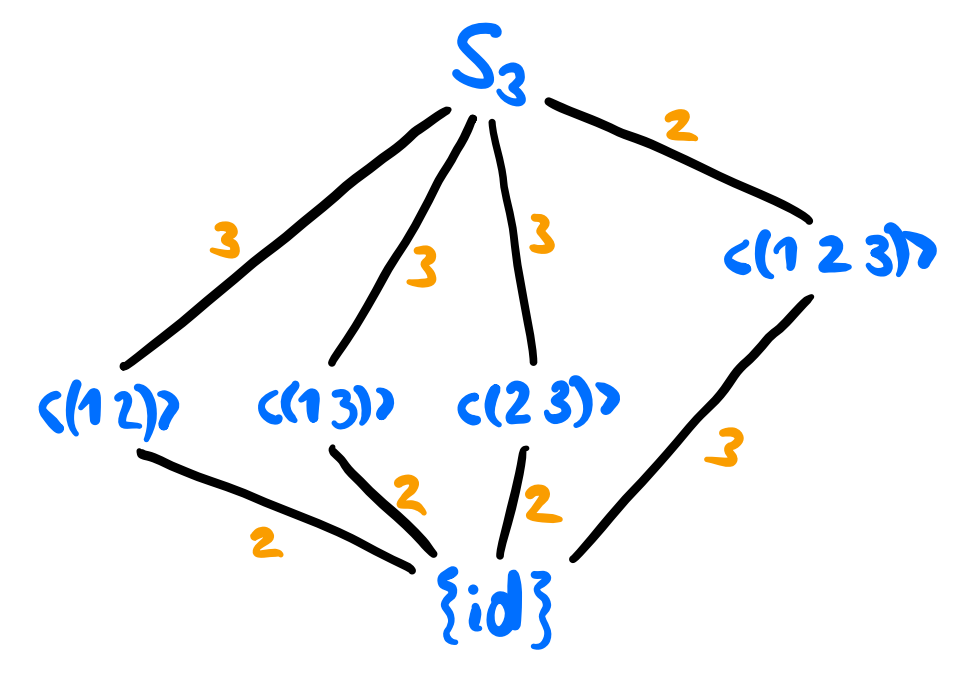
\includegraphics[width=\textwidth]{s3_subgroup_graph_index.png}
    \caption{Subgroup graph of the symmetric group $S_3$. The index of the subgroups is shown in orange.}
\end{marginfigure}

\begin{ex}{Normal subgroups (continued)}{}
\begin{itemize}
    \item $A_n \normal S_n$ as $A_n = \ker{\sgn}$, see \cref{eq:alternating_group}
    \item $\SL{n}{\R} \normal \GL{n}{\R}$ as $\SL{n}{\R} = \ker{\det}$, see \cref{eq:det_kernel}
    \item ${\Inn{G} \defeq \{i_g \mid g \in G\}}$ known as the \emph{inner automorphism group}\index{inner automorphism group} is a normal subgroup of the automorphism group, $\Inn{G} \normal \Aut{G}$
    \item For the symmetric group $S_3$, we have the normal subgroups \begin{itemize}
        \item $\{e\}, G \normal G$
        \item $A_3 = \gen{(1\ 2\ 3)} \normal G$
    \end{itemize} by \cref{lem:normal_subgroup_c}. Simple calculations confirm that the subgroups of order 2 are not normal.
\end{itemize}
\end{ex}

\begin{thm}[Quotient Group]\label{thm:quotient_group}
Let $N \normal G$. Then the set \begin{align}
    \Quot{G}{N} \defeq \{a N \mid a \in G\}
\end{align} is a group under the operation, \begin{align}
    a N \cdot b N \defeq (a \cdot b) N \quad \forall a, b \in G. \label{eq:quotient_group_op}
\end{align} $\Quot{G}{N}$ is called the \emph{quotient group}\index{quotient group} $G$ modulo $N$.
\end{thm} Thus, the quotient group is the group of (left) cosets of a normal subgroup. In particular, if $G$ is finite, we have, \begin{align}
    |\Quot{G}{N}| = \Index{G}{N} = \frac{|G|}{|N|},
\end{align} due to the \hyperref[defn:index]{definition of the index} and \hyperref[thm"lagrange]{Lagrange's theorem}. \begin{proof}
In proving that $\Quot{G}{N}$ is a group, we will see why we need the restriction of normal subgroups.

\begin{itemize}
    \item First, we need to show that the group operation \eqref{eq:quotient_group_op} is well-defined. Let us fix $a_1, a_2, b_1, b_2 \in G$ such that $a_1 N = a_2 N$ and $b_1 N = b_2 N$. We need to show $a_1 b_1 N = a_2 b_2 N$.
    
    As $N$ contains the neutral element $e$, we know $a_1 \in a_1 N$ and $a_2 \in a_2 N$. Therefore, $\exists n \in N.\ a_1 = a_2 n$ and, analogously, $\exists \Tilde{n} \in N.\ b_1 = b_2 \Tilde{n}$. We have, \begin{align*}
        a_1 b_1 = a_2 n b_2 \Tilde{n} = a_2 b_2 (\inv{b_2} n b_2 \Tilde{n}).
    \end{align*} Using that $N$ is normal, $\inv{b_2} n b_2 \in N$. Then, as $N$ is a subgroup, we also have $\inv{b_2} n b_2 \Tilde{n} \in N$. This shows that $a_1 b_1 N = a_2 b_2 N$.
    \item $e N = N$ is the neutral element.
    \item The group operation is closed under $\Quot{G}{N}$ by definition.
    \item $\inv{(a N)} = \inv{a} N$ clearly is the inverse of $a N$.
\end{itemize} $\implies \Quot{G}{N}$ is a group.
\end{proof}

\begin{ex}{Residue classes}{}
We will consider the quotient group $\Quot{\Z}{n\Z}$ of the group $(\Z,+)$ for any fixed $n \in \NZ$. We write, \begin{align}
    n\Z \defeq \gen{n} = \{n \cdot k \mid k \in \Z\}.
\end{align}

Observe that the left cosets are of the form \begin{align}
    a + n\Z = \{a + n \cdot k \mid k \in \Z\}.
\end{align} They are also called \emph{residue classes}\index{residue classes} modulo $n$.

To specify $\Quot{\Z}{n\Z}$, we are interested in finding when ${a + n\Z = b + n\Z}$ holds. We have, \begin{align}
    a + n\Z = b + n\Z \overset{\ref{lem:cosets_eq}}{\iff} a - b \in n\Z \overset{\ref{eq:left_coset}}{\iff} \divides{n}{a - b}.
\end{align} Equivalently to ${\divides{n}{a - b}}$, we say that $a$ is \emph{congruent}\index{congruent} $b$ modulo $n$ (denoted ${a \equiv b \mod n}$). For ${n > 0}$ this is equivalent to $a$ and $b$ having the same residue ${r \in \{0, 1, \dots, n - 1\}}$ when dividing by $n$.

From now on, we will assume ${n > 0}$. We denote elements by \begin{align}
    \rep{a} \defeq a + n\Z,
\end{align} where $a$ is referred to as the \emph{representative}\index{representative} of $\rep{a}$. It follows that, \begin{align}
    \Quot{\Z}{n\Z} = \{\rep{0}, \rep{1}, \dots, \rep{n-1}\}.
\end{align} By \cref{thm:quotient_group}, $\Quot{\Z}{n\Z}$ with the mapping ``$+$'' is a cyclic group of order $n$. It is often denoted by \begin{align}
    Z_n \defeq \Quot{\Z}{n\Z} = \gen{\rep{1}}.
\end{align}

As an example, consider $Z_8 = \{\rep{0}, \rep{1}, \rep{2}, \rep{3}, \rep{4}, \rep{5}, \rep{6}, \rep{7}\}$. We have, \vspace{-10pt}\begin{itemize}
    \item $\rep{2} + \rep{5} = \rep{7}$,
    \item $\rep{2} + \rep{6} = \rep{8} = \rep{0}$, and
    \item $\rep{-6} = \rep{2}$.
\end{itemize}
\end{ex}

\begin{defn}[Cokernel]
The \emph{cokernel}\index{cokernel} of a homomorphism ${\varphi : G \to H}$ is the quotient group $\Quot{H}{\im{\varphi}}$.
\end{defn}

\begin{ex}{Outer automorphism group}{}
Automorphisms that are not inner automorphisms are called \emph{outer automorphisms}\index{outer automorphism}. The \emph{outer automorphism group}\index{outer automorphism group} is the group of cosets of the inner automorphism group with respect to outer automorphisms, \begin{align}
    \Out{G} \defeq \Quot{\Aut{G}}{\Inn{G}}.
\end{align}

Let us define the homomorphism ${\sigma : G \to \Aut{G}, g \mapsto i_g}$. It can be shown that \vspace{-10pt}\begin{itemize}
    \item $\ker{\sigma} = Z(G)$,
    \item $\im{\sigma} = \Inn{G}$, and
    \item the cokernel of $\sigma$ is $\Out{G} = \Quot{\Aut{G}}{\Inn{G}}$.
\end{itemize}
\end{ex}
